\chapter{Позднеантичное наводнение}

\section{Место}
Сегодня я вам расскажу про крупнейшее наводнение в истории Италии, датированное 589 годом нашей эры. Случившееся, как и принято в этой рубрике, по причине эффективного менеджмента. 

\begin{figure}[h!tb]
	\centering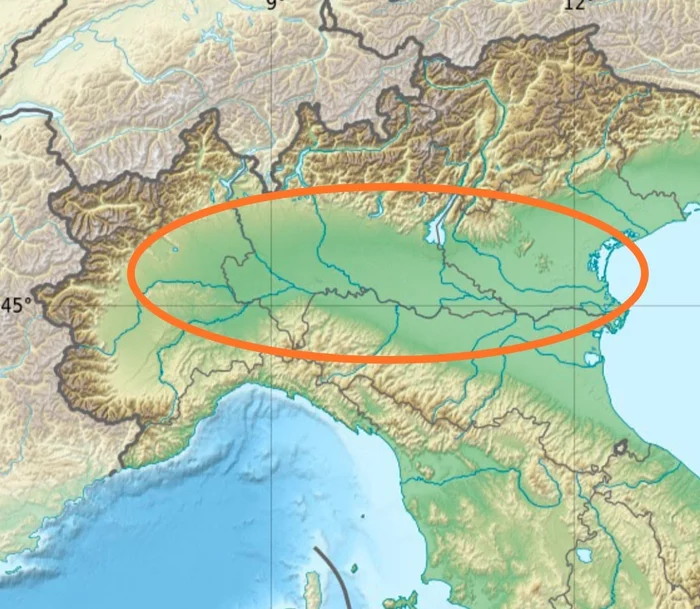
\includegraphics[scale=0.4]{Data/antic_technocrash/1614663824140324608.png}
	\caption{Вон там была техногенка. Первая карта
	}
	\label{fig:tech1} % Unique label used for referencing the figure in-text
	%\addcontentsline{toc}{figure}{Figure \ref{fig:placeholder}} % Uncomment to add the figure to the table of contents
\end{figure}



Большую часть Северной Италии занимает Паданская низменность, смотри первую карту. Это, преимущественно, бассейн реки По и десятков еë притоков и оттоков, несущих воду из Альп в Адриатику. 500 км в длину и 200 в ширину. Плодородный край, способный кормить всю Италию. Там тепло, много воды, хорошие почвы, а реки создавали естественные системы орошения. Правда, реки иногда вели себя неадекватно, выходили из берегов, меняли русла, сносили города. В общем - рискованное земледелие как оно есть. Но уже в позднереспубликанский период, выкинув отсюда всяких галлов и заселив Цизальпийскую Галлию своими ветеранами, римляне начинают укрощать природу, с любовью создавая огромную и очень сложную систему дамб, дренажных каналов и всего такого. Паданская низменность имеет уклон к морю, поэтому задачка была сложной. Но римляне справились. И уже в имперские времена постоянно развивали и усложняли систему, превратив регион в этакий итальянский огород для всего сапога.


В общем, носились римляне с этим регионом прям как египтяне со своим Нилом, считая необходимым держать у себя под боком источник продовольствия.




\section{Обстоятельства}
\begin{figure}[h!tb]
	\centering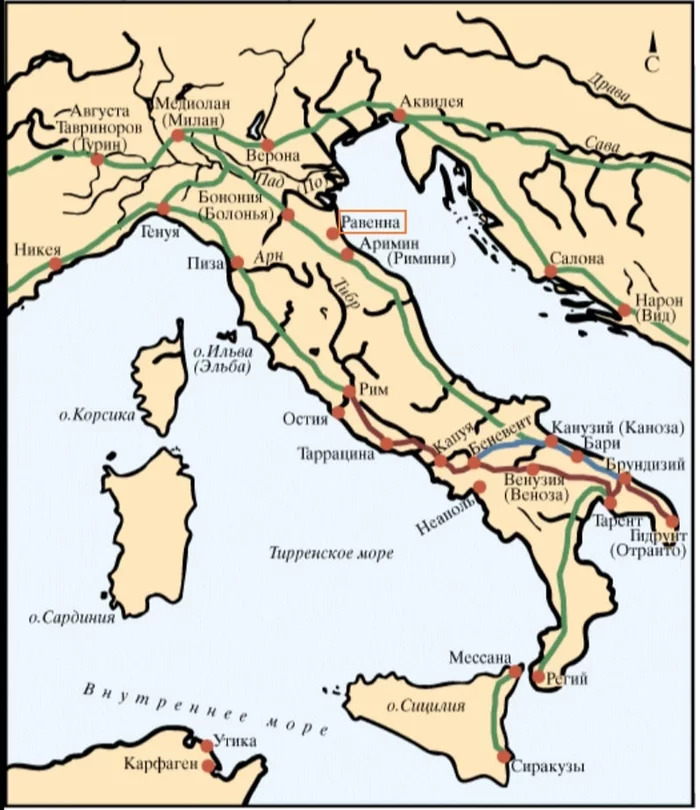
\includegraphics[scale=0.4]{Data/antic_technocrash/1614663828122115735.jpg}
	\caption{Вторая карта
	}
	\label{fig:tech2} % Unique label used for referencing the figure in-text
	%\addcontentsline{toc}{figure}{Figure \ref{fig:placeholder}} % Uncomment to add the figure to the table of contents
\end{figure}

А потом империя посыпалась. Почему - вопрос отдельный. Но там всем стало резко не до поддержания плотин в пригодном для использования состоянии. Сначала посыпались провинции, а затем и до Италии руки дошли. Только Рим сжигали дважды, в 410 и 455 годах, превратив город-миллионник в пепел с населением в пару тысяч человек, копающих грядки на руинах бывшего мегаполиса. "Все дороги ведут в Рим", как известно. Это было хорошо пока империя тягала по ним легионы, но когда по тем же дорогам начали бродить варварские орды - транспортная доступность стала очень большой проблемой. За пятый век в Италию вламывались вестготы, остготы, вандалы, бургунды и гунны. Причем если последних обьединенными усилиями както сумели забороть и выкинуть, то все остальные не столько грабили, сколько завоевывали и оседали на захваченных землях. Последние императоры сидели в Равенне (вторая карта) и старались не отсвечивать, выбрав этот город просто потомушта он был чуть в стороне от основных дорог, и поэтому варварам до него было далеко и неудобно идти. Но когда "первичный передел" Италии начал подходить к концу, то и до Равенны руки дошли, канешно же.


В общем, творился Адъ и Израиль. Не совсем уж тотальная резня, канешн (гуннов, кстати, за это и грохнули, за то что они жгли и уничтожали вообще всë, что для практичных варваров-федератов было дико и противоестественно), но ничего хорошего. Одоакр свергает последнего императора, потом остгот Теодорих сносит Одоакра и захватывает всю Италию, затем Юстиниан посылает Велирисария снести остготов, что тот успешно двадцать лет осуществляет. Бардак продолжается, а за плотинами никто не смотрит, они ветшают и всем на них плевать.


Затем в Италию вламываются лангобарды, отбивают весь север сапога и начинают завоевывать остальное. И вот тут КАК ЕБАНЕТ!




\section{Результаты}

Тут есть две версии. Либо "оно само" случилось, либо хитрые лангобарды хотели чуть-чуть подкрутить русло одной из рек, чтоб осложнить византийцам переброску войск. Но, в любом случае, при местечке Кукко (современное название Веронелла) что-то пошло ОЧЕНЬ сильно не так, и масса воды и грязи с огромной скоростью понеслась к морю, меняя ландшафт до неузнаваемости. Римское ирригационное наследие настолько обветшало, что по "эффекту домино" сель понесся вниз, прошел около ста километров до побережья и вылился в Адриатическое море, намыв тем самым дополнительные 12 квадратных километров земли (третья карта. На четвертой видно расстояние по прямой, а кружком - то, как наводнение поменяло прибрежную линию). 


Последствия были ужасающими. Людей погибла целая куча, Падую отрезало от остальной Италии, а то, что раньше было плодородным краем, превратилось в болото на многие столетия. Те, кто выжил в этом рукотворном Апокалипсисе, по большей части предпочли мигрировать на север, в Венецианскую комунну. Которая позже станет Светлейшей Республикой Венеция. 
\begin{figure}[h!tb]
	\centering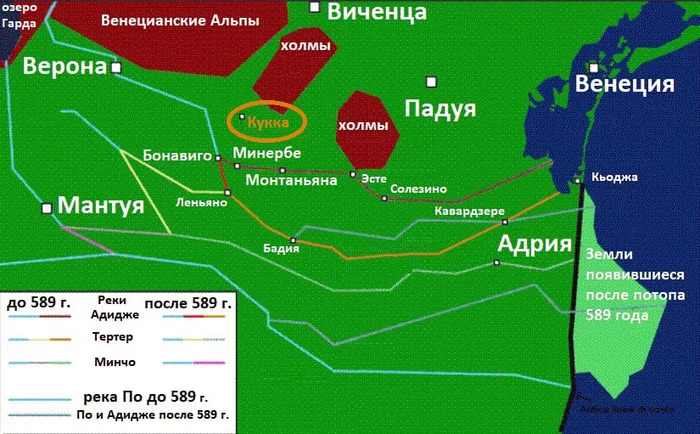
\includegraphics[scale=0.5]{Data/antic_technocrash/1614663830115017356.jpg}
	\caption{Третья карта
	}
	\label{fig:tech3} % Unique label used for referencing the figure in-text
	%\addcontentsline{toc}{figure}{Figure \ref{fig:placeholder}} % Uncomment to add the figure to the table of contents
\end{figure}

\begin{figure}[h!tb]
	\centering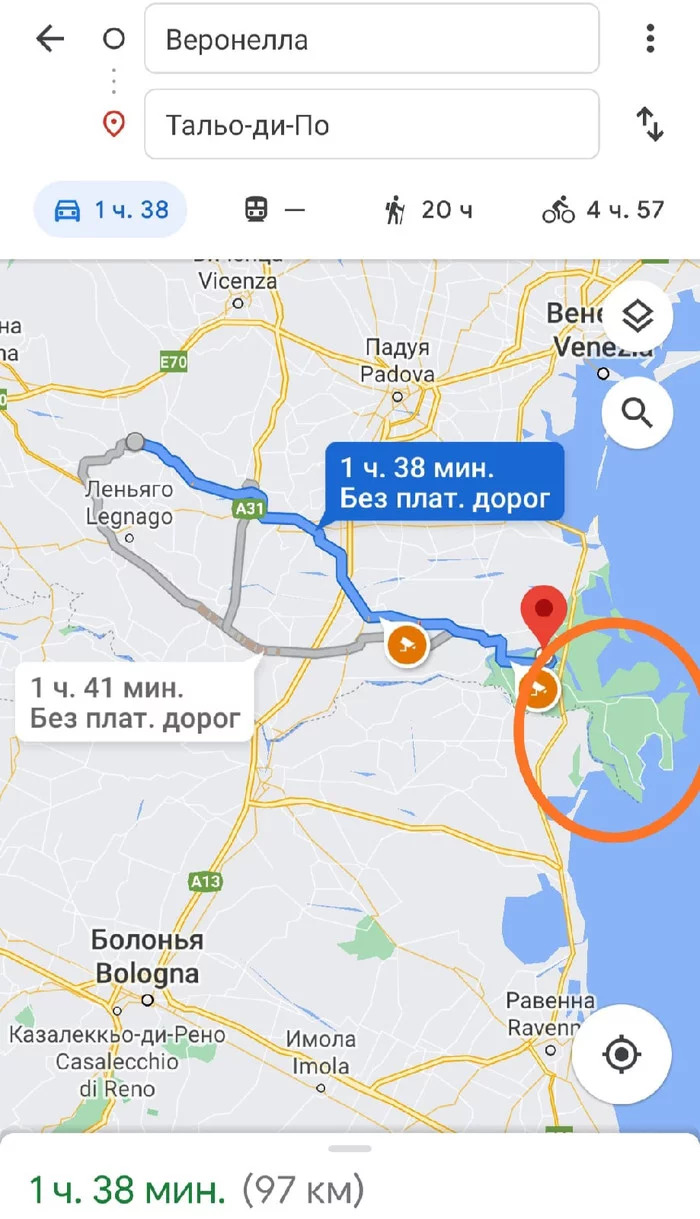
\includegraphics[scale=0.3]{Data/antic_technocrash/1614663836179610411.jpg}
	\caption{Четвертая карта
	}
	\label{fig:tech4} % Unique label used for referencing the figure in-text
	%\addcontentsline{toc}{figure}{Figure \ref{fig:placeholder}} % Uncomment to add the figure to the table of contents
\end{figure}
Пожалуй, венецианцы это главное наследие того наводнения, и именно из-за него они вообще состоялись как явление. Следите за руками.


У коренного населения Италии весь этот варварский постапокалипсис никакого энтузиазма не вызывал. И заныкаться от него куда подальше было их давней мечтой. Мы уже говорили про Равенну, которую избрали столицей в пятом веке так как она была в стороне от проторенных маршрутов и имела выход в Адриатику, что давало возможность контактировать с Восточной Римской Империей. Равенну в итоге взяли, но мечта заныкаться куда-нибудь в болото не отпускала истинных римлян, и они как раз где-то в этом регионе и оседали, преимущественно. Особенно после вторжения лангобардов, которые последовательно вышибали Византию из Италии. И как раз в это время происходит наводнение, которое:


\begin{itemize}
	\item Лишает крова и средств к существованию огромное количество людей в пострадавших областях. Многие погибли, канешн, но многие и выжили. А всë нажитое непосильным трудом было потеряно и у тех и у других.
	\item  Превращает огромную территорию в практически непроходимое болото и отрезает северо-восточный кусок Италии от остального сапога.
	\item  Выжившие, а это, преимущественно те, кто успел за последние годы пожить под византийцами, понимают, что у них теперь два путя. Либо идти под лангобардов, в более открытые места, либо наоборот, забиваться в ещë большее болото, чтобы сраные варвары уж точно не достали.
\end{itemize}

Так, собственно, из преимущественно латинского населения, и формируется костяк будущей Республики. В конце концов, через пару десятков лет, после одной чумы и одного арабского нашествия, Византия теряет все свои завоевания, кроме как раз-таки Венеции. Которая для сухопутной армии была, благодаря своей географии, неприступной крепостью, а с моря они были прикрыты собственным флотом и Византией. А так как выращивать жратву там было невозможно в силу всë той же географии, люди там жили морем, преимущественно морской торговлей и морским разбоем, быстро став в этих вопросах признанными мастерами.


Вот такая история. 